\documentclass[12pt,a4paper]{article}
\usepackage[utf8]{inputenc}
\usepackage[T2A]{fontenc}
\usepackage[russian]{babel}
\usepackage{amsmath, amsthm, amssymb}
\usepackage[left=2cm,right=2cm,top=2cm,bottom=2cm]{geometry}
\usepackage{indentfirst}

% Красивое оформление содержания
\usepackage{hyperref}

\title{\textbf{Конспект к коллоквиуму по математическому анализу}}
\author{Николаев Всеволод}

\begin{document}

\maketitle

\tableofcontents


\newpage
\section{Равномерная непрерывность. Примеры. Теорема Кантора о равномерной непрерывности.}

\subsection{Используемые понятия}
% ===== sub_1.tex =====
% Вспомогательные определения/теоремы, НЕ являющиеся центральными,
% но необходимые для доказательства (компакт, непрерывность, и т.д.)

\textbf{Компакт в $\mathbb{R}$.}
Множество $K\subset\mathbb{R}$ называется \emph{компактным}, если оно \emph{замкнуто} и \emph{ограничено}.

\medskip

\textbf{Определение непрерывной функции (точечное).}
Функция $f$ непрерывна в $x_0$, если
\[
\forall \varepsilon>0\;\exists \delta>0:\;
|x-x_0|<\delta \;\Longrightarrow\;
|f(x)-f(x_0)|<\varepsilon.
\]
Если это верно для каждой точки множества $X$, говорят, что $f$ непрерывна на $X$.

\medskip

\textbf{Теорема о сходящейся подпоследовательности (Больцано--Вейерштрасса).}
Всякая \emph{ограниченная} последовательность в $\mathbb{R}$ имеет \emph{сходящуюся} подпоследовательность.  
Если $(x_n)$ лежит в компактном $K$, то любая подпоследовательность $(x_{n_k})$ имеет сходящуюся подпоследовательность с пределом в $K$.  


\subsection{Ответ на вопрос}
\textbf{Условие:}
Является ли линейным пространством множество матриц \( 2 \times 2 \) со следом \( 1 \)?

\textbf{Решение:}
Рассмотрим множество всех матриц \( 2 \times 2 \) со следом 1:

\[
V = \{ A \in M_{2 \times 2} \mid \text{tr}(A) = 1 \}
\]

где \( \text{tr}(A) \) обозначает след матрицы \( A \), т.е. сумму элементов на главной диагонали.

Чтобы проверить, является ли \( V \) линейным пространством, проверим основные свойства линейного пространства: замкнутость относительно сложения и умножения на скаляр.

\textbf{Проверка замкнутости относительно сложения:}  
Если \( A, B \in V \), то их сумма \( A + B \) должна также принадлежать \( V \), то есть иметь след, равный 1.

\[
\text{tr}(A + B) = \text{tr}(A) + \text{tr}(B).
\]

Так как по условию \( \text{tr}(A) = 1 \) и \( \text{tr}(B) = 1 \), то:

\[
\text{tr}(A + B) = 1 + 1 = 2.
\]

Но \( 2 \neq 1 \), следовательно, \( A + B \notin V \), и множество \( V \) не замкнуто относительно сложения.

\textbf{Проверка замкнутости относительно умножения на скаляр:}  
Пусть \( A \in V \) и \( \lambda \) — произвольное число. Тогда проверим, принадлежит ли \( \lambda A \) множеству \( V \):

\[
\text{tr}(\lambda A) = \lambda \text{tr}(A) = \lambda \cdot 1 = \lambda.
\]

Так как при произвольном \( \lambda \) значение \( \text{tr}(\lambda A) \) может быть любым, оно не обязательно равно 1. Следовательно, \( \lambda A \notin V \), и множество \( V \) не замкнуто относительно умножения на скаляр.

\textbf{Вывод:}  
Так как множество \( V \) не замкнуто ни относительно сложения, ни относительно умножения на скаляр, оно \textbf{не является линейным пространством}.



\newpage
\section{Дифференциал функции. Теорема Ферма. Теорема Ролля. Примеры.}

\subsection{Используемые понятия}
% ===== sub_2.tex =====
% Вспомогательные факты, не являющиеся центральными в основном вопросе
% но используемые в доказательствах (локальный экстремум, теорема Вейерштрасса и т.д.)

\textbf{Локальный экстремум.}
Точка $x_0$ называется \emph{локальным минимумом} (соответственно, максимумом), если существует $\delta>0$ такое, что для всех $x$ из $(x_0-\delta, x_0+\delta)$ выполняется $f(x)\ge f(x_0)$ (или $f(x)\le f(x_0)$ для максимума).

\medskip

\textbf{Теорема Вейерштрасса (о достижении экстремума).}
Если $f$ непрерывна на отрезке $[a,b]$, то $f$ достигает на нём своих наибольшего и наименьшего значений. Формально:
\[
\exists x_{\min}, x_{\max}\in[a,b]:\quad
f(x_{\min}) \le f(x) \le f(x_{\max})
\quad
\forall x \in [a,b].
\]

\textbf{Производная в точке.}
Напомним, $f'(x_0)$ есть предел
\[
\lim_{x\to x_0}\frac{f(x)-f(x_0)}{x - x_0},
\]
если этот предел конечен.


\subsection{Ответ на вопрос}
\subsection{Расчёт средних значений углов и параметра \(a\)}

В таблицах 1–3 приведены по три независимых измерения углов \(\alpha_{m,i}\) для каждого порядка
\[
	m = 0, \pm1, \pm2, \pm3
\]
и для трёх спектральных линий (\(i=1\) — красная, \(i=2\) — зелёная, \(i=3\) — фиолетовая).

Для каждого цвета \(i\) и каждого порядка \(m\) выполняются следующие шаги:
\begin{enumerate}
	\item Вычисление среднего угла
	      \[
		      \bar\alpha_{m,i}
		      = \frac{1}{3}\sum_{k=1}^{3}\alpha_{m,i}^{(k)}.
	      \]
	\item Определение углового смещения относительно центрального максимума (\(m=0\)):
	      \[
		      \varphi_{m,i}
		      = \bar\alpha_{m,i} \;-\; \bar\alpha_{0,i}.
	      \]
	\item Расчёт параметра
	      \[
		      a_{m,i}
		      = \frac{\sin\varphi_{m,i}}{m},
		      \qquad m\neq 0.
	      \]
\end{enumerate}



\newpage
\section{Теорема Лагранжа. Необходимoе и достаточное условие постоянства дифференцируемой функции на промежутке. Необходимое и достаточное условие монотонности дифференцируемой функции на промежутке.}

\subsection{Используемые понятия}
% ===== sub_3.tex =====
% Вспомогательный файл: содержит факты/определения, не являющиеся
% центральной частью вопроса, но нужные в доказательствах.

\textbf{Теорема Ролля (напоминание).}
Пусть $f$ непрерывна на $[a,b]$, дифференцируема на $(a,b)$ и $f(a)=f(b)$. Тогда существует точка $c\in(a,b)$, где $f'(c)=0$.

\textbf{Определение дифференцируемости (напоминание).}
Функция $f$ называется дифференцируемой в точке $x_0$, если существует конечный предел
\[
f'(x_0) = \lim_{x\to x_0} \frac{f(x)-f(x_0)}{x - x_0}.
\]
Если $f'(x_0)$ существует для всех $x_0$ в $(a,b)$, говорят, что $f$ дифференцируема на $(a,b)$.

\textbf{Определение монотонности (напоминание).}
Функция $f$ называется \emph{возрастающей} на $(a,b)$, если для любых $x_1,x_2\in(a,b)$, при $x_1 < x_2$ выполняется $f(x_1)\le f(x_2)$ (нестрого) или $f(x_1)<f(x_2)$ (строго).  
Аналогично определяется убывание.

\textbf{Определение постоянной функции.}
Функция $f$ называется постоянной на $(a,b)$, если $f(x_1)=f(x_2)$ для любых $x_1,x_2\in(a,b)$.

% (Другие напоминания (о непрерывности, ...) при необходимости).


\subsection{Ответ на вопрос}
\subsection{Оценка погрешности \(\bar a_i\)}

По каждому цвету \(i\) (красный, зелёный, фиолетовый) собрана выборка из \(N=6\) значений параметра
\[
	a_{i,m} = \frac{\sin\varphi_{i,m}}{m}\,, \quad m=\pm1,\pm2,\pm3.
\]

Для оценки результата косвенного измерения \(a_i\) и его погрешности при доверительной
вероятности \(P=95\%\) используем выборочный метод:
\[
	\bar a_i = \frac{1}{N}\sum_{k=1}^N a_{i,k},
	\qquad
	S_i = \sqrt{\frac{1}{N-1}\sum_{k=1}^N\bigl(a_{i,k}-\bar a_i\bigr)^2},
\]
\[
	\Delta\bar a_i = t_{0.95,\,N-1}\,\frac{S_i}{\sqrt{N}}.
\]

Затем результат оформляется в виде
\(\displaystyle a_i = \bar a_i \pm \Delta\bar a_i\)
и заносится в Таблицу 5.


\newpage
\section{Равномерная непрерывность. Примеры. Теорема Кантора о равномерной непрерывности.}

\subsection{Используемые понятия}
% ===== sub_4.tex =====
% Вспомогательные определения и теоремы,
% не являющиеся центральными в данном вопросе,
% но используемые в доказательстве теоремы Кантора

\textbf{Определение компакта в $\mathbb{R}$.}
Множество $K\subset\mathbb{R}$ называется \emph{компактным}, если оно \emph{замкнуто} и \emph{ограничено}.

\medskip

\textbf{Теорема Болльцано--Вейерштрасса.}
Всякая \emph{ограниченная} последовательность $(x_n)$ в $\mathbb{R}$ имеет \emph{сходящуюся} подпоследовательность.  
На языке компактных множеств: любая последовательность, целиком лежащая в компактном $K$, содержит сходящуюся подпоследовательность с пределом в $K$.

\medskip

\textbf{Определение непрерывности (подробно).}
Напомним: $f$ непрерывна на $X$, если для любой точки $x_0\in X$:
\[
\forall \varepsilon>0\;\;\exists \delta>0:\;
|x - x_0|<\delta \implies |f(x)-f(x_0)|<\varepsilon.
\]

\medskip

% (Другие напоминания и определения — при необходимости).


\subsection{Ответ на вопрос}
\subsection{Построение и аппроксимация зависимости \(\sin\varphi_m\) от \(m\)}

Для каждой спектральной линии (\(i=1\) — красная, \(i=2\) — зелёная, \(i=3\) — фиолетовая) были рассчитаны точки
\[
	\bigl(m,\;\sin\varphi_{m,i}\bigr),
	\quad m=\pm1,\pm2,\pm3,
\]
и построены аппроксимирующие прямые
\[
	\sin\varphi = a_i\,m
\]
методом наименьших квадратов без свободного члена. Ниже приведены соответствующие графики.

\begin{figure}[H]
	\centering
	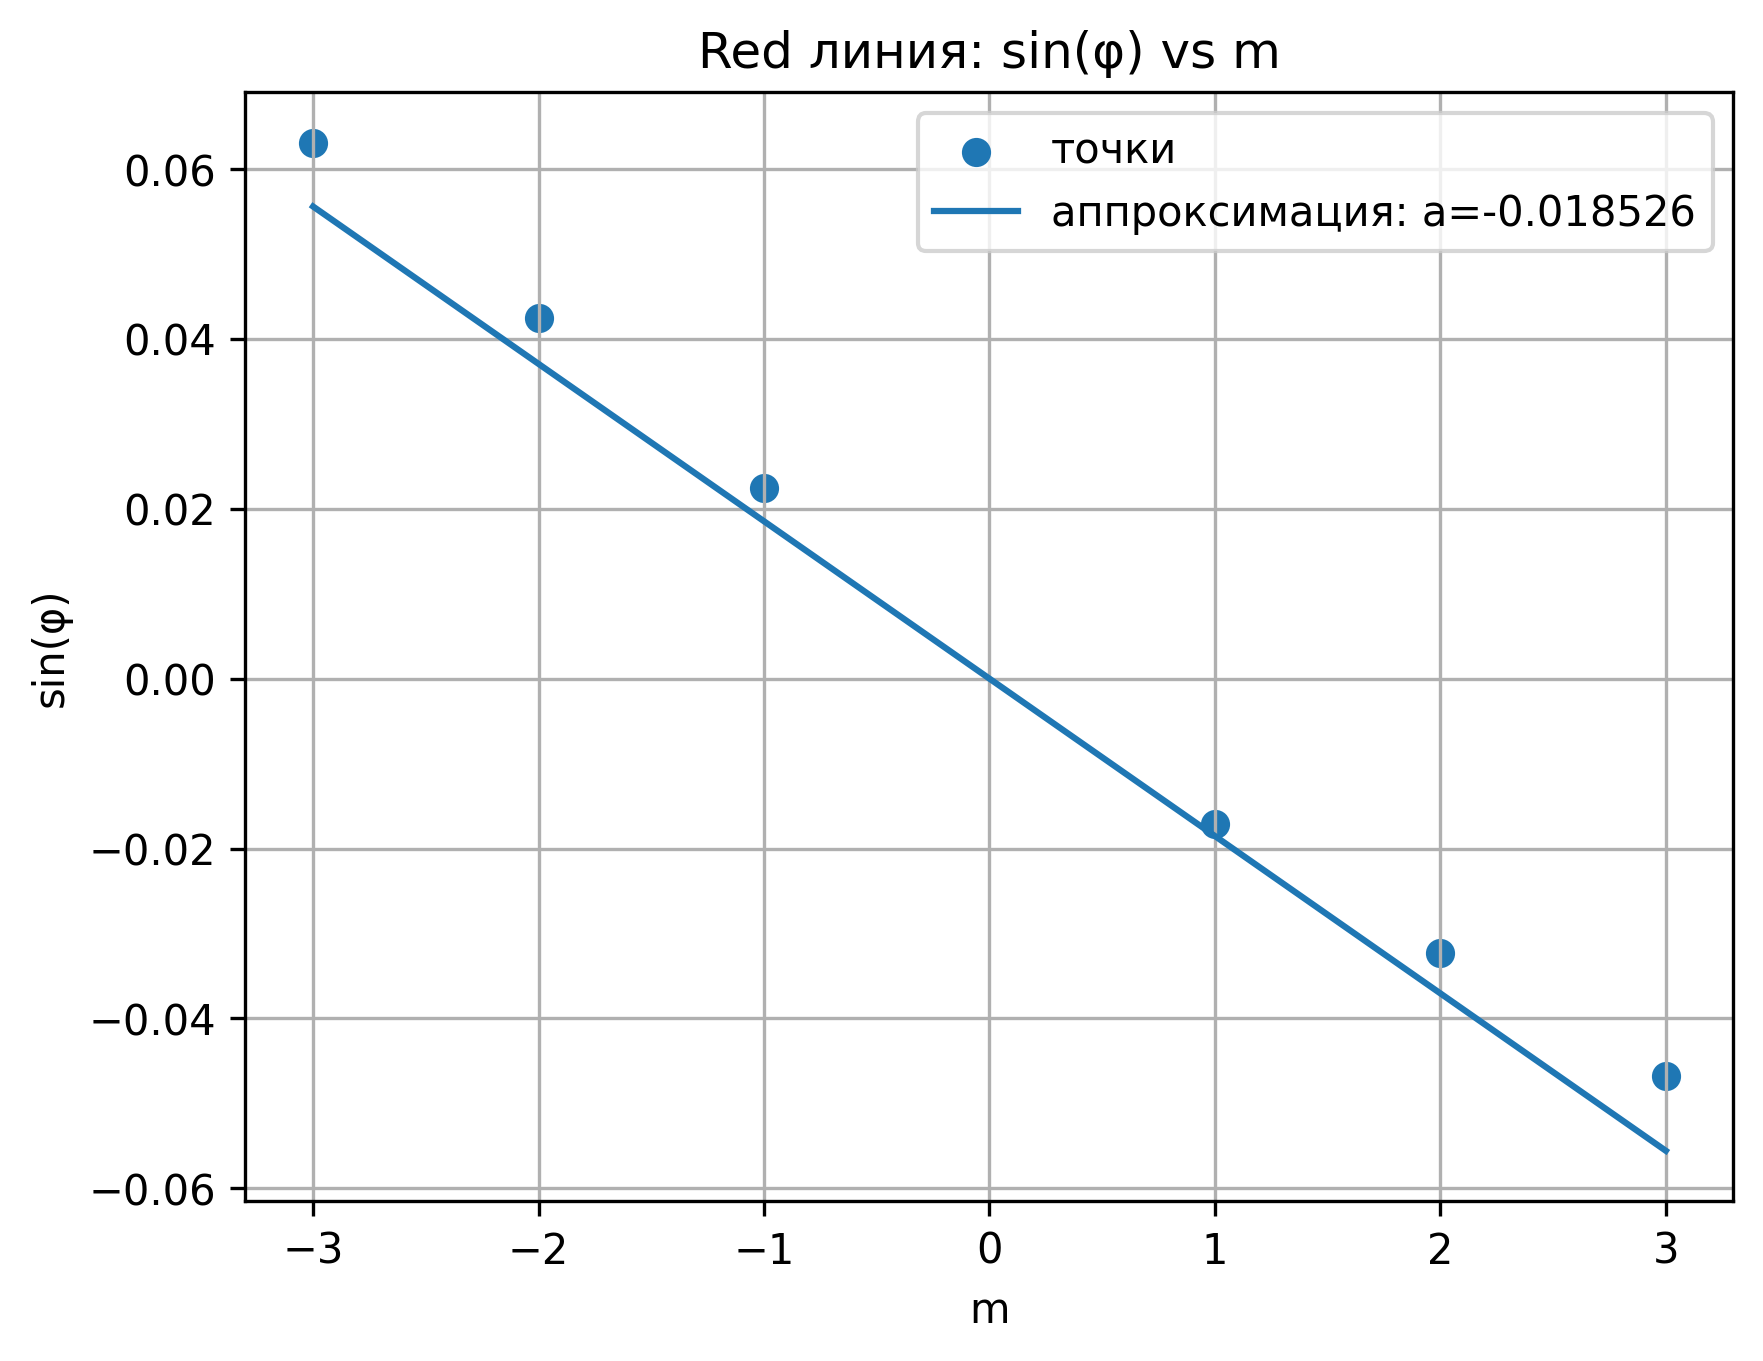
\includegraphics[width=0.7\textwidth]{images/red_fit.png}
	\caption{Красная линия: \(\sin\varphi\) vs.\ \(m\) и аппроксимация \(a_1\,m\).}
	\label{fig:sinphi-red}
\end{figure}

\begin{figure}[H]
	\centering
	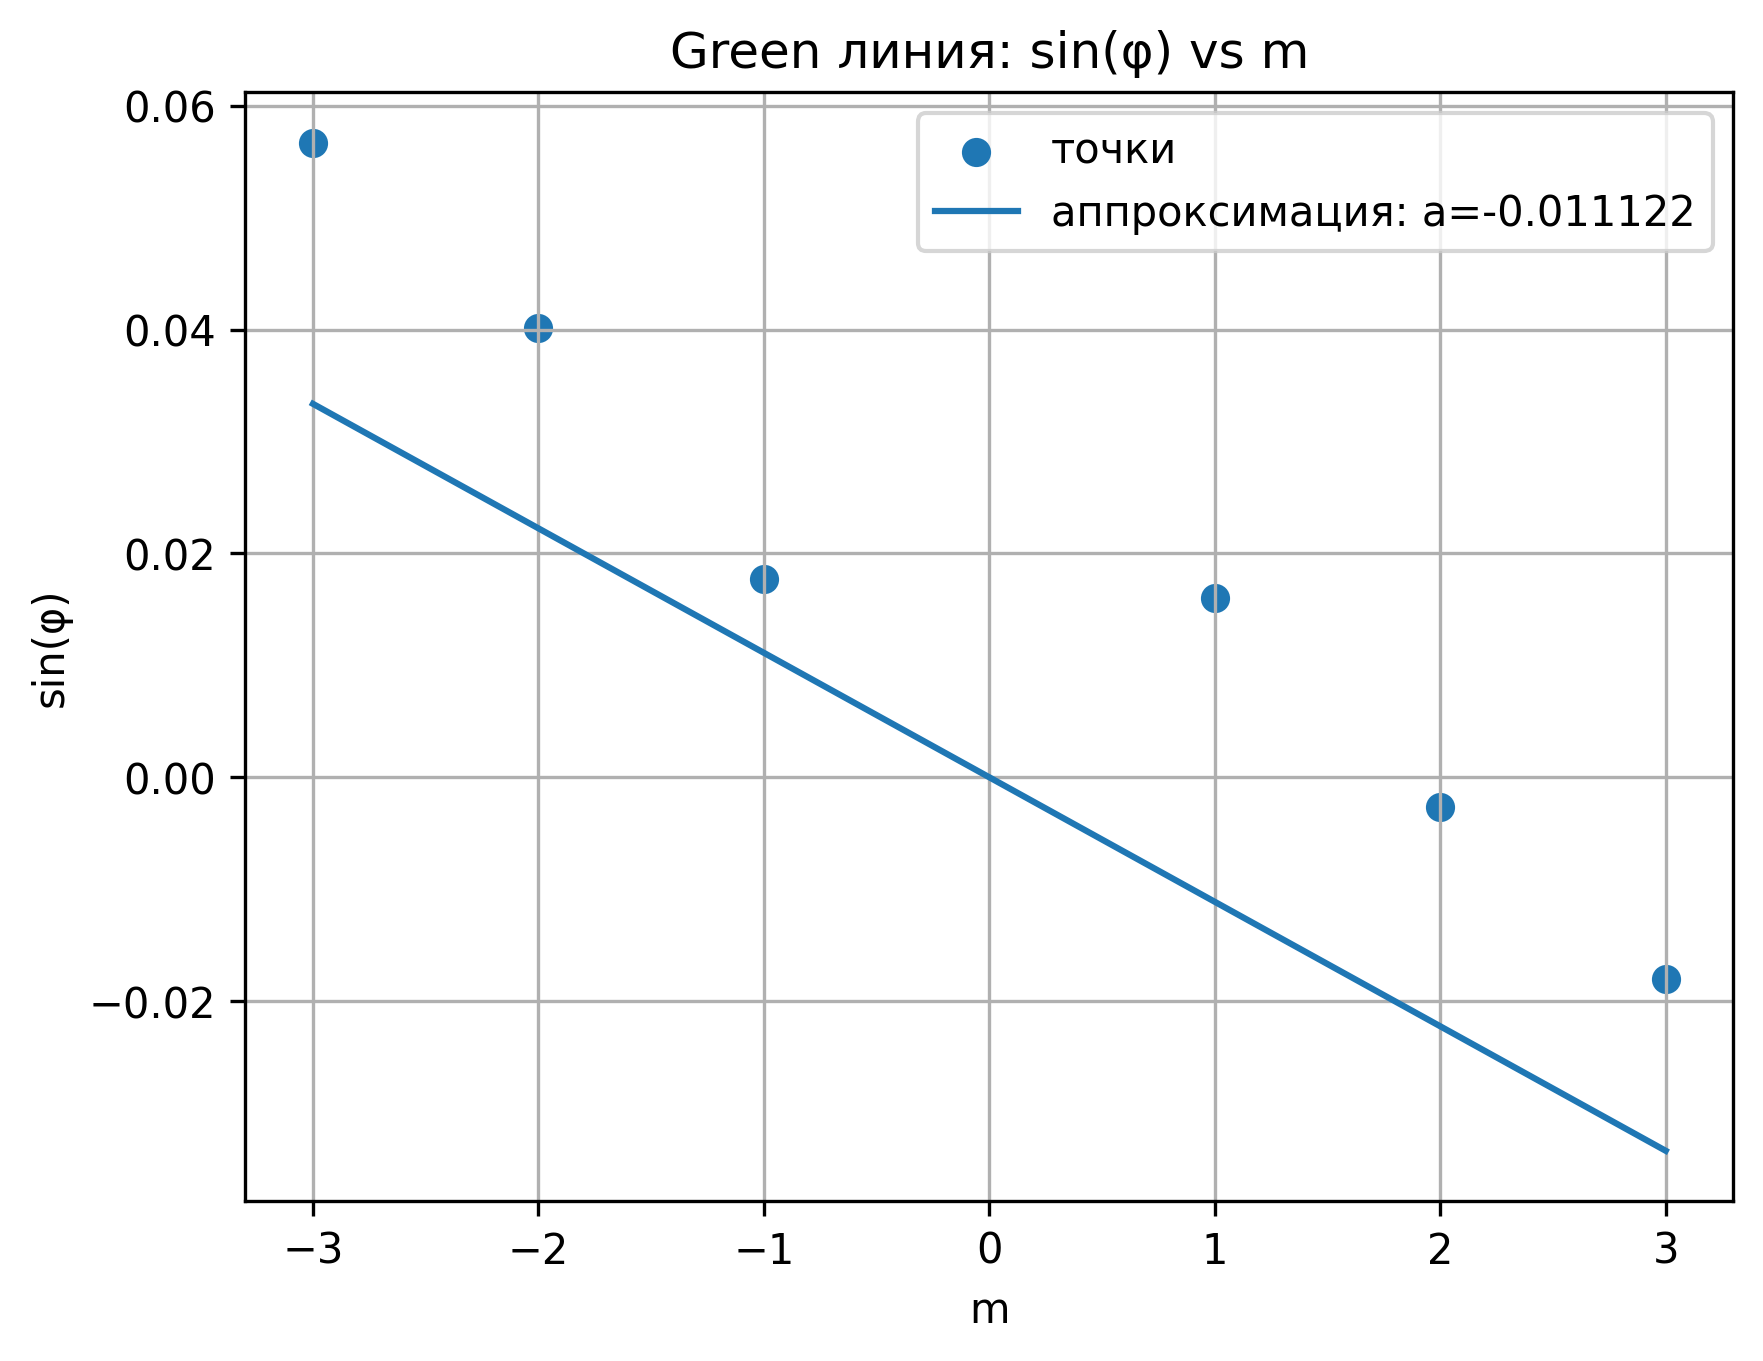
\includegraphics[width=0.7\textwidth]{images/green_fit.png}
	\caption{Зелёная линия: \(\sin\varphi\) vs.\ \(m\) и аппроксимация \(a_2\,m\).}
	\label{fig:sinphi-green}
\end{figure}

\begin{figure}[H]
	\centering
	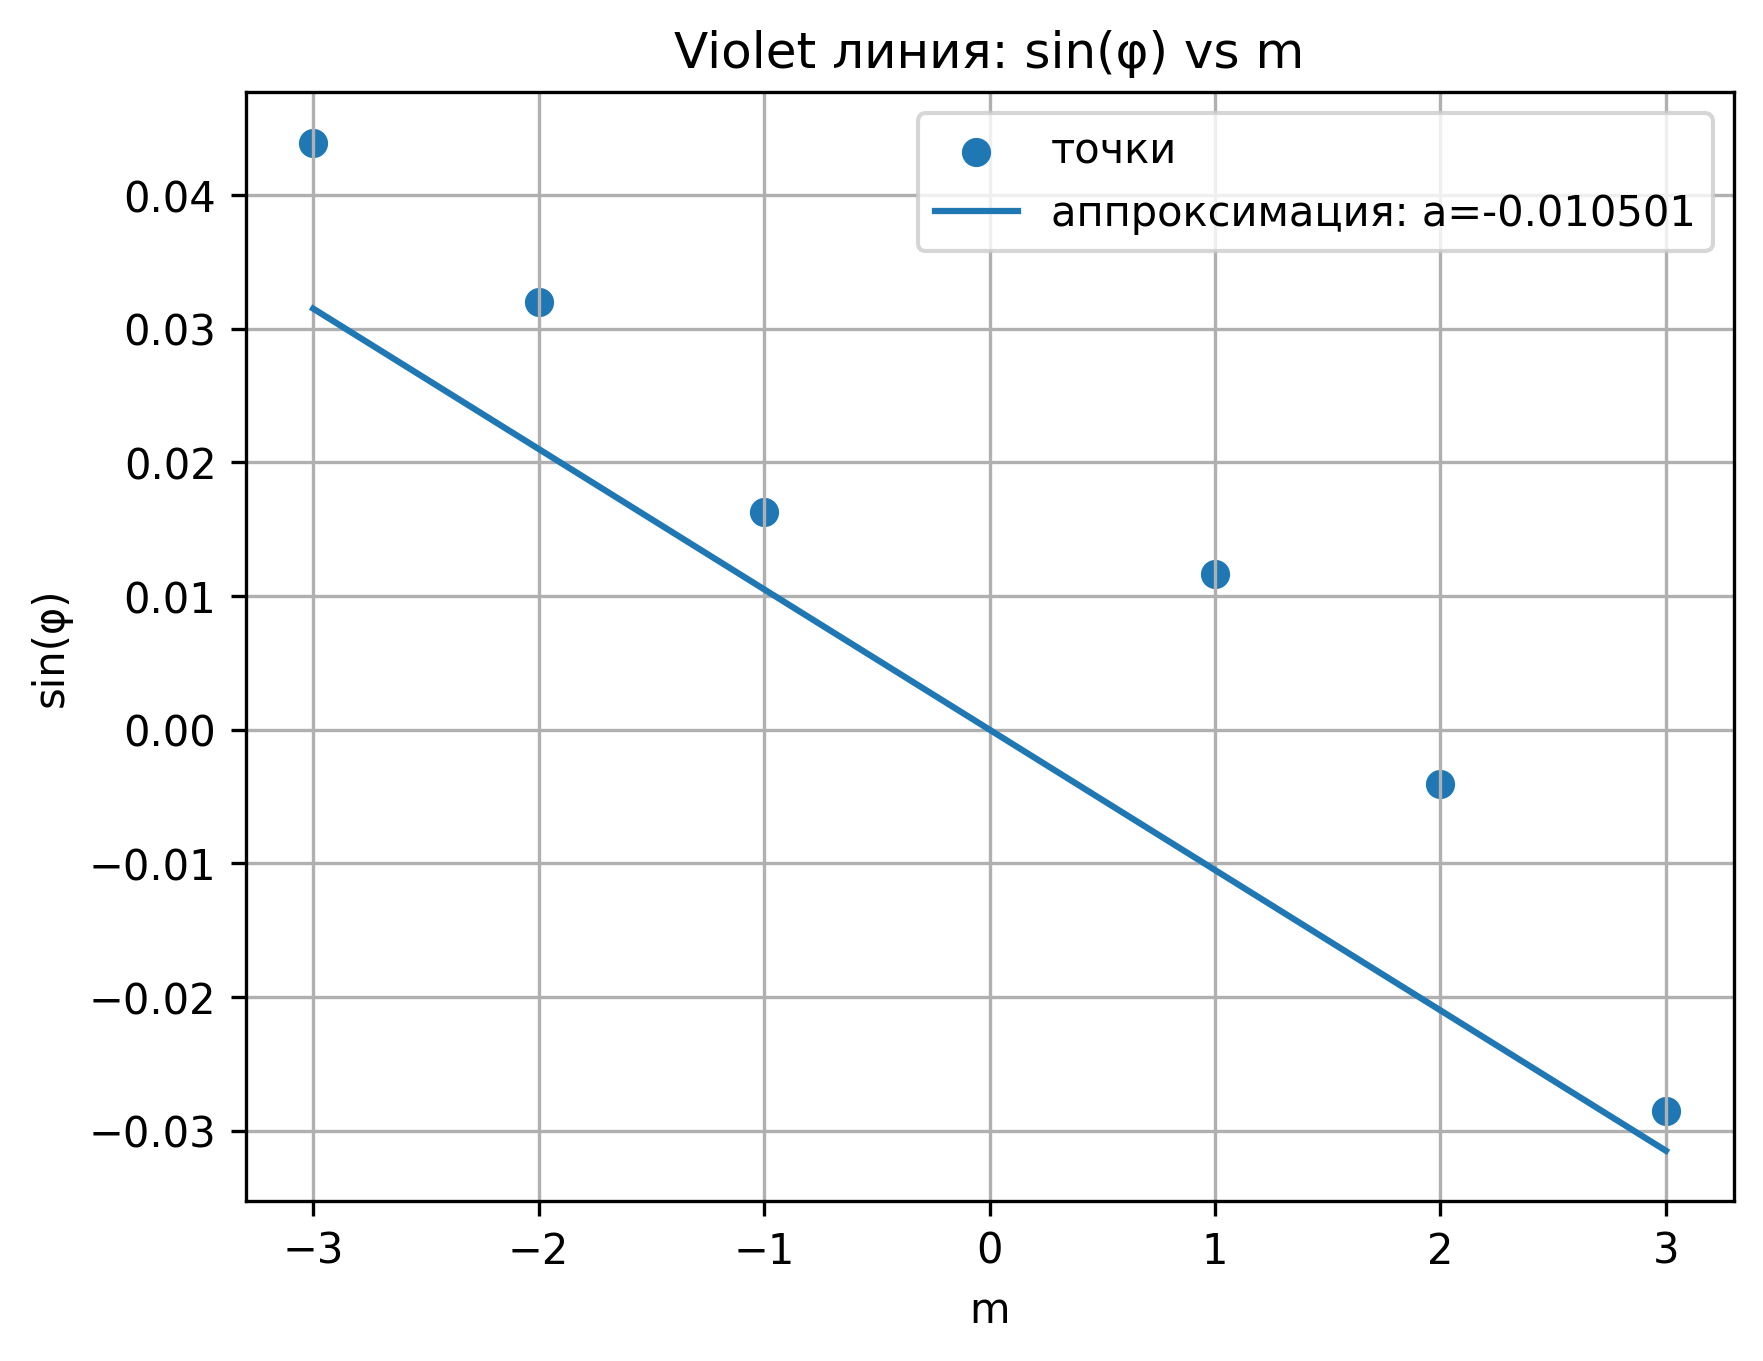
\includegraphics[width=0.7\textwidth]{images/violet_fit.png}
	\caption{Фиолетовая линия: \(\sin\varphi\) vs.\ \(m\) и аппроксимация \(a_3\,m\).}
	\label{fig:sinphi-violet}
\end{figure}


\newpage
\section{Вывод рядов Тейлора для функций y=exp(x), y=sinx, y=cosx через следствие из теоремы Лагранжа. Формула Эйлера.}

\subsection{Используемые понятия}
% ===== sub_5.tex =====
% Вспомогательный файл: факты, не являющиеся центральными в данном вопросе,
% но нужные при доказательствах (теорема Лагранжа, определение (n+1)-й производной и т.п.)

\textbf{Теорема Лагранжа (о среднем значении).}
Пусть функция $f$ непрерывна на $[0,x]$ (при $x>0$) и дифференцируема на $(0,x)$. Тогда существует $c\in(0,x)$ такое, что
\[
f(x)-f(0) \;=\; f'(c)\,\bigl(x - 0\bigr).
\]

\medskip

\textbf{n-я производная.}
Функция $f$ называется $n$ раз дифференцируемой в точке, если существуют все производные $f'(x_0), f''(x_0),\dots,f^{(n)}(x_0)$. Аналогично в окрестности.

\medskip

\textbf{Определение комплексной экспоненты (для Формулы Эйлера).}
Если $z$ комплексное, $e^z$ определяется как \(\sum_{n=0}^{\infty}\frac{z^n}{n!}\). Это расширяет понятие экспоненты на комплексную область.


\subsection{Ответ на вопрос}
\subsection{Постоянная решётки \(d\)}

Используем табличное значение длины волны зелёной линии
\[
	\lambda_2 = 546 \pm 5\ \text{нм}\quad(P=95\%),
\]
и средний угловой коэффициент
\[
	a_2 = \bar a_2 \pm \Delta\bar a_2,
\]
где \(\bar a_2\) и \(\Delta\bar a_2\) получены в п.~3 (см. Таблицу 5).
Тогда
\[
	d = \frac{\lambda_2}{\lvert \bar a_2\rvert},
	\qquad
	\Delta d = d \,
	\sqrt{\Bigl(\tfrac{\Delta \lambda_2}{\lambda_2}\Bigr)^2
		+\Bigl(\tfrac{\Delta \bar a_2}{\bar a_2}\Bigr)^2}\,.
\]

Результат занесён в таблицу 4.


\newpage
\section{Теорема Коши. Правило Лопиталя (доказательство – только для случая 0/0). Примеры, когда правило неприменимо.}

\subsection{Используемые понятия}
% ===== sub_6.tex =====
% Вспомогательные определения/теоремы, не являющиеся
% "центральными" в данном вопросе, но используемые в доказательствах.

\textbf{Теорема Ролля (напоминание).}
Пусть $f$ непрерывна на отрезке $[p,q]$, дифференцируема на $(p,q)$ и $f(p)=f(q)$. Тогда существует точка $c\in(p,q)$, где $f'(c)=0$.

\medskip

\textbf{Определение: проколотая окрестность.}
Говорят, что функция $f$ дифференцируема (или определена) в проколотой окрестности точки $a$, если существует $\delta>0$ такое, что при $0<|x-a|<\delta$, $f(x)$ (и её производная) определена. При этом в самой точке $a$ она может быть не определена или не дифференцируема.

\medskip

\textbf{Неопределённости вида $0/0$ и $\infty/\infty$.}
Правило Лопиталя распространяется на случаи, когда \(\lim_{x\to a}f(x)=\lim_{x\to a}g(x)=0\) или \(\pm\infty\). В остальных случаях правило не даёт результата.



\subsection{Ответ на вопрос}
\subsection{Длины волн красного и фиолетового}

Используем формулы
\[
	\lambda_i = a_i\,d,
	\qquad
	\Delta\lambda_i = \lambda_i
	\sqrt{\Bigl(\tfrac{\Delta d}{d}\Bigr)^2 + \Bigl(\tfrac{\Delta a_i}{a_i}\Bigr)^2},
	\quad i = 1,3,
\]
где \(a_i\pm\Delta a_i\) и \(d\pm\Delta d\) взяты из предыдущих пунктов.
Результаты занесены в Таблицу 5.


\newpage
\section{Формула Тейлора для многочлена. Формула Тейлора с остатком в форме Пеано.}

\subsection{Используемые понятия}
% ===== sub_7.tex =====
% Вспомогательный файл: определения/факты, не являющиеся центральной частью вопроса,
% но нужные при доказательствах (например, "n-кратная дифференцируемость", "o( (x-x0)^n )" и т. п.)

\textbf{Определение n-кратной дифференцируемости.}
Функция $f$ называется $n$ раз дифференцируемой в точке $x_0$, если существуют конечные все производные $f'(x_0), f''(x_0), \dots, f^{(n)}(x_0)$.

\medskip

\textbf{Малое «о» и запись $o(g(x))$.}
Говорят, что $h(x)$ есть $o\bigl(g(x)\bigr)$ при $x\to x_0$, если
\[
\lim_{x\to x_0}\frac{h(x)}{g(x)} = 0.
\]
В таком случае пишут $h(x)=o(g(x))$.

\medskip

\textbf{Остаточный член в форме Лагранжа (напоминание).}
Если $f$ имеет $(n+1)$-ю производную в окрестности $x_0$, то для
\[
f(x) = f(x_0) + \dots + \frac{f^{(n)}(x_0)}{n!}(x - x_0)^n + R_n(x)
\]
справедливо
\[
R_n(x) = \frac{f^{(n+1)}(\xi)}{(n+1)!}(x - x_0)^{n+1},\quad \xi \in (x_0,x).
\]



\subsection{Ответ на вопрос}
\subsection*{Определение угловой дисперсии \(D_{\varphi}\)}

Угловая дисперсия решётки определяется из уравнения (4.5):
\[
	D_{\varphi} \;=\;\frac{d\varphi}{d\lambda}
	\;=\;\frac{m}{d\,\cos\varphi_m}\,,
\]
где \(\varphi_m\) — угловое смещение для порядка \(m\), \(d\) — постоянная решётки (в тех же единицах, что и длина волны \(\lambda\)).
В отчёте \(D_{\varphi}\) выражается в угловых единицах (минутах) на нанометр. Для этого результат переводят из радиан на минуты:
\[
	D_{\varphi}\bigl[\tfrac{\text{угл. мин}}{\text{нм}}\bigr]
	= \frac{m}{d\cos\varphi_m}\times\frac{180\cdot60}{\pi}\,.
\]
Рассчитанные значения занесены в Таблицу 5.


\newpage
\section{Достаточные условия существования экстремума (по второй производной).}

\subsection{Используемые понятия}
% ===== sub_8.tex =====
% Вспомогательные определения/теоремы, не являющиеся центральными в данном вопросе,
% но требующиеся в доказательствах (например, теорема Ферма).

\textbf{Теорема Ферма (напоминание).}
Если $f$ дифференцируема в точке $x_0$ и имеет там локальный экстремум, то $f'(x_0)=0$.

\medskip

\textbf{Определение непрерывности второй производной.}
Если $f''(x)$ существует в некоторой окрестности $x_0$ и является непрерывной в $x_0$, то говорят, что $f$ имеет \emph{непрерывную вторую производную} в $x_0$.

\medskip

\textbf{Дифференцируемость в $(a,b)$.}
Говорят, что $f$ дифференцируема на интервале $(a,b)$, если $f'(x)$ существует для всех $x\in(a,b)$.


\subsection{Ответ на вопрос}
% ===== 8.tex =====
% "Достаточные условия существования экстремума (по второй производной)."

% 1. Определения

\textbf{Локальный минимум и максимум.}
Точка $x_0$ внутри промежутка $(a,b)$ называется \emph{точкой локального минимума} функции $f$, если существует $\delta>0$, что для всех $x$ с $|x-x_0|<\delta$ выполняется
\[
f(x)\;\ge\;f(x_0).
\]
Аналогично, $x_0$ является \emph{точкой локального максимума}, если в некоторой окрестности $x_0$ значение $f(x)\le f(x_0)$.

\medskip

\textbf{Вторая производная.}
Если функция $f$ дифференцируема на $(a,b)$, и $f'(x)$ тоже дифференцируема на $(a,b)$, то в точках, где это возможно, определена \emph{вторая производная} $f''(x)$.

\medskip

% 2. Теоремы и ключевые утверждения

\textbf{Теорема (достаточные условия экстремума по второй производной).}
Пусть $f$ дифференцируема на $(a,b)$ и $x_0 \in (a,b)$ — такая точка, где $f'(x_0)=0$. Предположим, что у $f$ существует непрерывная в $x_0$ вторая производная $f''(x_0)$. Тогда:
\begin{enumerate}
  \item Если $f''(x_0)>0$, то $x_0$ — точка \textbf{локального минимума}.
  \item Если $f''(x_0)<0$, то $x_0$ — точка \textbf{локального максимума}.
  \item Если $f''(x_0)=0$, вывод не делается (нужен дополнительный анализ).
\end{enumerate}

\medskip

% 3. Основные идеи доказательства (коротко)

\begin{itemize}
  \item Ключевой «трюк»: если $f''(x_0)>0$, то $f'(x)$ возрастает вблизи $x_0$. Но при $x_0$ мы имеем $f'(x_0)=0$.  
  \item Следовательно, для $x>x_0$, $f'(x)$ становится положительной (или почти), а для $x<x_0$ — отрицательной (или почти), что даёт локальный минимум.  
  \item Аналогично, если $f''(x_0)<0$, $f'(x)$ убывает вблизи $x_0$, и $x_0$ — локальный максимум.
\end{itemize}

\medskip

% 4. Полное доказательство (по шагам, ссылаясь на sub_8 при необходимости)

\textbf{Доказательство достаточности (подробно):}

\begin{enumerate}
  \item \textbf{Наличие $f'(x_0)=0$.}  
    По \textbf{теореме Ферма} (см. \texttt{sub\_8.tex}), это условие часто является необходимым для экстремума. Мы рассматриваем \emph{достаточность}, когда вдобавок знаем про вторую производную.
  \item \textbf{Случай $f''(x_0)>0$.}  
    \begin{itemize}
      \item Из непрерывности $f''$ в $x_0$ вытекает, что при $x$ достаточно близком к $x_0$, вторая производная $f''(x)$ «сохраняет» тот же знак (положительный).  
      \item Значит $f'(x)$ строго возрастает вблизи $x_0$. Но $f'(x_0)=0$.  
      \item Тогда для $x>x_0$ с $x$ рядом с $x_0$, $f'(x)$ станет положительной, а для $x<x_0$ — отрицательной.  
      \item Следовательно, при $x>x_0$, $f$ возрастает, при $x<x_0$, $f$ убывает. Значит $x_0$ — локальный минимум.
    \end{itemize}
  \item \textbf{Случай $f''(x_0)<0$.}  
    \begin{itemize}
      \item Аналогичные рассуждения: $f'(x)$ вблизи $x_0$ будет убывать, и при $x>x_0$ произведёт знак отрицательный, а при $x<x_0$ — знак положительный (около $x_0$).  
      \item Следовательно, слева функция возрастает, а справа убывает. Точка $x_0$ — локальный максимум.
    \end{itemize}
  \item \textbf{Случай $f''(x_0)=0$.}  
    \begin{itemize}
      \item Из этого факта \emph{нельзя} вывести строгое заключение об экстремуме: нужны дополнительные рассуждения (см. примеры $x^3$, $x^4$).
    \end{itemize}
\end{enumerate}

\medskip

% 5. Примеры

\begin{itemize}
  \item \emph{Функция $f(x)=x^2$:}  
  $f'(0)=0$, $f''(0)=2>0$. По теореме, $x=0$ — локальный минимум (что верно).
  \item \emph{Функция $f(x)=x^3$:}  
  $f'(0)=0$, $f''(0)=0$. По рассматриваемой теореме вывод не делается, и действительно $x=0$ — точка перегиба, \textit{не} экстремум.
  \item \emph{Функция $f(x)=-x^2$:}  
  $f'(0)=0$, $f''(0)=-2<0$. Значит в $x=0$ локальный максимум.
\end{itemize}

\medskip

% -- Логическая связность (определения в sub_8.tex)


\newpage
\section{Теорема Лиувилля. Пример трансцендентного числа.}

\subsection{Используемые понятия}
% ===== sub_9.tex =====
% Вспомогательные определения и факты,
% не являющиеся "центральными" в вопросе, но используемые в доказательстве

\textbf{Минимальный многочлен алгебраического числа.}
Пусть $\alpha$ — алгебраическое (корень целого ненулевого многочлена). Его \emph{минимальным многочленом} называется многочлен $P(x)\in \mathbb{Z}[x]$, у которого $\alpha$ — корень, степень $P$ — наименьшая возможная, и старший коэффициент положителен, а все общие делители коэффициентов равны 1.

\medskip

\textbf{Оценка "разности корней".}
Из теории алгебраических уравнений известно, что если $P(x)$ — многочлен степени $d$ с целыми коэффициентами, то расстояния между его корнями не могут быть «слишком маленькими» относительно высоты коэффициентов. Точнее, если $r_1,\dots,r_d$ — корни, то существуют нижние границы $|r_i-r_j|$ в зависимости от коэффициентов $P$ (см. теорему о разложении в произведение линейных множителей).

\medskip

\textbf{Рациональное приближение.}
Если $\alpha$ действительно алгебраична степени $d$, то для больших $q$ рациональные приближения $\frac{p}{q}$ не могут удовлетворять $|\alpha - \frac{p}{q}| < \tfrac{1}{q^n}$ при $n>d$, иначе возникнет противоречие (Теорема Лиувилля).


\subsection{Ответ на вопрос}
\subsection{Разрешающая способность \(R\)}

Разрешающая способность решётки определяется по формуле
\[
	R = m\,N,
\]
где \(m\) — порядок спектра, а \(N\) — число штрихов решётки (см. п.~8).
Для \(m=1\) и \(m=3\) получаем:
\[
	R_1 = 1 \times N,\quad R_3 = 3 \times N.
\]

Результаты занесены в Таблицу 5.


\newpage
\section{Формулы Маклорена для функций y=exp(x), y=sinx, y=cosx, y=ln(1+x), y=pow((1+x),a).}

\subsection{Используемые понятия}
% ===== sub_10.tex =====
% Вспомогательные определения и факты,
% не являющиеся "центральными" в вопросе,
% но требующиеся при доказательствах (n-я производная, radius of convergence и т.п.)

\textbf{Определение n-й производной.}
Если функция $f$ $n$ раз дифференцируема в окрестности 0, то $f^{(n)}(0)$ есть её $n$-я производная в точке 0.

\medskip

\textbf{Радиус сходимости степенного ряда.}
Ряд $\sum_{n=0}^{\infty} c_n x^n$ имеет некий \emph{радиус сходимости} $R$, $0\le R\le \infty$, где ряд сходится при $|x|<R$ и расходится (как правило) при $|x|>R$.

\medskip

\textbf{Бином Ньютона (обобщённый).}
Для вещественного $a$ при $|x|<1$:
\[
(1+x)^a = \sum_{n=0}^{\infty} \binom{a}{n}\,x^n,
\]
где $\displaystyle \binom{a}{n} = \frac{a(a-1)\dots(a-n+1)}{n!}$.

\medskip

\textbf{Формула Тейлора (общая).}
При разложении $f(x)$ в окрестности 0 с учётом всех производных получаем ряд (если сходится) называемый рядом Маклорена, частный случай ряда Тейлора.


\subsection{Ответ на вопрос}
\subsection{Минимальный различимый интервал \(\Delta\lambda\)}

Минимальный интервал длин волн, который может разрешить решётка, рассчитывается по критерию Рэлея:
\[
	\Delta\lambda = \frac{\lambda}{R},
\]
где \(\lambda\) — средняя длина волны линии, \(R\) — разрешающая способность (см. п.~9).

Результаты приведены в Таблице 5.


\newpage
\section{Формула Тейлора с остатком в форме Лагранжа. Приближенные вычисления по формуле Тейлора.}

\subsection{Используемые понятия}
% ===== sub_11.tex =====
% Вспомогательный файл: определения и теоремы, не являющиеся центральными
% в вопросе, но используемые при доказательствах (Теорема Коши/Ролля в обобщённом виде, ...
% понятие n-кратной производной).

\textbf{Обобщённая теорема Ролля (Теорема Коши).}
Если $f$ и $g$ непрерывны на $[a,b]$, дифференцируемы на $(a,b)$, и $g'(x)\neq 0$ на $(a,b)$, то существует $c\in(a,b)$:
\[
\frac{f(b)-f(a)}{g(b)-g(a)} = \frac{f'(c)}{g'(c)}.
\]
При удачном выборе «вспомогательных» функций подстановка даёт нужный результат о $F^{(n+1)}(\xi)=0$.

\medskip

\textbf{n-кратная производная в точке.}
Если $f$ дифференцируема $n$ раз в окрестности $x_0$, мы обозначаем $f^{(n)}(x_0)$ как производную $n$-го порядка, если та существует и непрерывна.

\medskip

\textbf{Пример применения индукции.}
Чтобы показать наличие $\xi$ с $F^{(n+1)}(\xi)=0$, обычно делают «по шагам»: сначала доказывают, что в $(a,b)$ есть $c_1$ с $F^{(1)}(c_1)=0$ (Теорема Ролля), затем в $(a_1,b_1)$ подинтервале ищут $c_2$ с $F^{(2)}(c_2)=0$, и т. д.


\subsection{Ответ на вопрос}
% ===== 11.tex =====
% "Формула Тейлора с остатком в форме Лагранжа. Приближённые вычисления по формуле Тейлора."

% 1. Определения

\textbf{Формула Тейлора и остаточный член.}
Пусть $f$ имеет $(n+1)$-ю производную в окрестности точки $x_0$. Тогда можно представить $f(x)$ в виде:
\[
f(x) = f(x_0) + \frac{f'(x_0)}{1!}\,(x - x_0) + \dots + \frac{f^{(n)}(x_0)}{n!}\,(x - x_0)^n + R_n(x),
\]
где $R_n(x)$ называется \emph{остаточным членом}.

\medskip

\textbf{Форма Лагранжа остаточного члена.}
Существует точка $\xi$ между $x_0$ и $x$ (включая возможность $\xi \in (x,x_0)$), такая что
\[
R_n(x) = \frac{f^{(n+1)}(\xi)}{(n+1)!}\,(x - x_0)^{n+1}.
\]
Это утверждение мы будем доказывать ниже (используя теорему Лагранжа о среднем значении).

\medskip

% 2. Теоремы и ключевые утверждения

\textbf{Формулировка (Тейлор + Лагранж).}
Пусть $f$ непрерывно дифференцируема на отрезке $[x_0,x]$ (или $[x,x_0]$) до порядка $(n+1)$. Тогда:
\[
f(x) = \underbrace{\sum_{k=0}^{n} \frac{f^{(k)}(x_0)}{k!}\,(x-x_0)^k}_{\text{многочлен Тейлора порядка }n} \;+\; \frac{f^{(n+1)}(\xi)}{(n+1)!}\,(x - x_0)^{n+1},
\]
где $\xi$ лежит между $x_0$ и $x$.

\medskip

\textbf{Приближённые вычисления.}
Чтобы вычислить $f(x)$ примерно, берут полином Тейлора степени $n$:
\[
P_n(x) = \sum_{k=0}^{n} \frac{f^{(k)}(x_0)}{k!}\,(x - x_0)^k,
\]
и оценивают ошибку (погрешность) через
\[
|R_n(x)| = \left|\frac{f^{(n+1)}(\xi)}{(n+1)!}\,(x - x_0)^{n+1}\right|.
\]
Обычно используют верхнюю оценку: если $|f^{(n+1)}(t)| \le M$ на $[x_0,x]$, то
\[
|R_n(x)| \;\le\; \frac{M\,|x - x_0|^{n+1}}{(n+1)!}.
\]

\medskip

% 3. Основные идеи доказательства (коротко)

\begin{itemize}
  \item Рассмотрим функцию $F(x) = f(x) - P_n(x)$, где $P_n(x)$ — многочлен Тейлора степени $n$ вокруг $x_0$.  
  \item По определению $P_n$, все производные $F$ до порядка $n$ в точке $x_0$ равны нулю.  
  \item Применяем теорему Лагранжа \textit{в обобщённом виде} (Теорема Коши или вариант теоремы Ролля) к $F$ на отрезке $[x_0,x]$, получаем существование точки $\xi$, где $(n+1)$-я производная $F^{(n+1)}(\xi)=0$. Но $F^{(n+1)}(t)=f^{(n+1)}(t)$, потому что $(n+1)$-я производная многочлена $P_n$ равна нулю.  
  \item Отсюда возникает
  \[
  F(x) = F(x_0) + \dots + \frac{F^{(n+1)}(\xi)}{(n+1)!} (x-x_0)^{n+1},
  \]
  но $F(x_0)=F'(x_0)=\dots=F^{(n)}(x_0)=0$. Значит $F(x)=\frac{f^{(n+1)}(\xi)}{(n+1)!}(x-x_0)^{n+1}$.
\end{itemize}

\medskip

% 4. Полное доказательство (шаги, ссылаясь на sub_11 если нужно)

\textbf{Шаг 1: Построение многочлена Тейлора.}
\[
P_n(t) \;=\; \sum_{k=0}^{n} \frac{f^{(k)}(x_0)}{k!}\,(t - x_0)^k.
\]
По определению производной порядок $k$, $P_n$ «согласован» с $f$ до $n$-го порядка в точке $x_0$.

\textbf{Шаг 2: Рассмотрим $F(t)=f(t) - P_n(t)$.}
Тогда
\[
F^{(k)}(x_0) = f^{(k)}(x_0) - P_n^{(k)}(x_0) = 0 \quad\text{для } k=0,1,\dots,n.
\]

\textbf{Шаг 3: Применяем обобщённую теорему Ролля.}
На отрезке $[x_0, x]$ (или $[x,x_0]$), функция $F$ удовлетворяет условию $F^{(k)}(x_0)=F^{(k)}(x) \dots$ (не все равны, но ключ в том, что мы можем включить вспомогательную функцию «$G(t)=\dots$» — см. \texttt{sub\_11.tex} о теореме Коши). В итоге \emph{по индукции} выводится, что существует $\xi$ между $x_0$ и $x$, где $F^{(n+1)}(\xi)=0$. А $F^{(n+1)}(t)=f^{(n+1)}(t)$.

\textbf{Шаг 4: Остаточный член.}
\[
F(x) = f(x)-P_n(x) = \frac{f^{(n+1)}(\xi)}{(n+1)!}\,(x - x_0)^{n+1}.
\]
Перенося, получаем:
\[
f(x)=P_n(x) + \frac{f^{(n+1)}(\xi)}{(n+1)!}\,(x - x_0)^{n+1}.
\]
Это и есть искомая формула Тейлора с остатком в форме Лагранжа.

\medskip

% 5. Пример приближённых вычислений

\textbf{Пример: функция $f(x)=\sqrt{1+x}$, при $x$ мало.}
\begin{itemize}
  \item Выбираем $x_0=0$. Имеем $f(0)=1$, $f'(0)=\tfrac12$, $f''(0)=-\tfrac{1}{8}$, \dots .
  \item Третьепорядочное приближение: 
  \[
    P_2(x)=1 + \frac12 x - \frac{1}{8} x^2.
  \]
  \item Ошибка (остаток) $R_2(x)=\frac{f^{(3)}(\xi)}{3!} x^3$ для некоторого $\xi \in (0,x)$.  
  Используя оценку $|f^{(3)}(t)|\le M$ на $[0,x]$, будет 
  \(\bigl|R_2(x)\bigr|\le \frac{M|x|^3}{6}.\)
\end{itemize}
Так можно оценить точность приближённого вычисления $\sqrt{1+x}\approx 1 + \tfrac12 x - \tfrac18 x^2$ для малых $x$.

\medskip

% -- Логическая связность --
% (Подробные определения "обобщённой теоремы Ролля", "f^{(k)}(x_0)", "непрерывность" и т.д. см. sub_11.tex)


\newpage
\section{Формула Стирлинга (с эквивалентностью).}

\subsection{Используемые понятия}
% ===== sub_12.tex =====
% Вспомогательные определения/теоремы, не являющиеся
% "центральными" в вопросе 12, но используемые в доказательстве
% (Формула Стирлинга (с эквивалентностью)).

\textbf{Интегральная аппроксимация суммы.}
Ключ к доказательству формулы Стирлинга:
\[
\sum_{k=1}^{n}\ln k
\quad \text{сравнивается с} \quad
\int_{1}^{n}\ln x \,dx.
\]
Разность между этой суммой и интегралом — «погрешность», часто контролируемая приёмами типа «прямоугольников» или \emph{упрощённой} формулы Эйлера–Маклорена.

\medskip

\textbf{Обозначения: } $O(\cdot), \; o(\cdot).$
Символ $O(g(n))$ означает, что рассматриваемая величина не превосходит по абсолютному значению $C\,|g(n)|$ при достаточно больших $n$.  
Символ $r(n)=o(g(n))$ значит \(\lim_{n\to\infty}\frac{r(n)}{g(n)}=0\).

\medskip

\textbf{Эквивалентность функций.}
Запись $f(n)\sim g(n)$ означает \(\lim_{n\to\infty}\frac{f(n)}{g(n)}=1\). 
В контексте формулы Стирлинга: \(n!\sim \sqrt{2\pi n}\,\bigl(\tfrac{n}{e}\bigr)^n\). 


\subsection{Ответ на вопрос}
% ===== 12.tex =====
% "Формула Стирлинга (с эквивалентностью)."

% 1. Определения

\textbf{Факториал $n!$.}
Для натурального $n$ вводится произведение:
\[
n! \;=\;1\cdot2\cdot\dots\cdot n.
\]

\medskip

\textbf{Формула Стирлинга (эквивалентность).}
При $n\to\infty$
\[
n! \;\sim\;\sqrt{2\pi\,n}\,\Bigl(\tfrac{n}{e}\Bigr)^n,
\]
то есть
\[
\lim_{n\to\infty}\frac{n!}{\sqrt{2\pi\,n}\,\bigl(\tfrac{n}{e}\bigr)^n}=1.
\]

\medskip

% 2. Теоремы и ключевые утверждения

\textbf{Основная идея.}
Используется:
\[
\ln(n!)=\sum_{k=1}^n\ln k
\quad\approx\quad
\int_{1}^{n}\ln x\,dx=n\ln n - n +1.
\]
Разность «сумма – интеграл» даёт поправку, которая приводит к множителю \(\sqrt{2\pi n}\).

\medskip

% 3. Полное доказательство (шаги)

\begin{enumerate}
  \item \textbf{Переход к логарифмам.}
    \[
      \ln(n!)=\sum_{k=1}^n\ln k.
    \]
  \item \textbf{Сравнение с интегралом.}
    \[
      \sum_{k=1}^n\ln k
      \;\approx\;\int_{1}^{n}\ln x\,dx
      = n\ln n - n + 1.
    \]
  \item \textbf{Тонкая оценка (через формулу Эйлера–Маклорена).}
    \[
      \ln(n!)=n\ln n - n +\tfrac12\ln(n)+O(1).
    \]
  \item \textbf{Экспоненцирование.}
    \[
      n!=\exp(n\ln n - n +\tfrac12\ln n +O(1))
      =\sqrt{n}\,\Bigl(\tfrac{n}{e}\Bigr)^n\,\exp\bigl(O(1)\bigr).
    \]
    При более точном разборе получается желаемый множитель \(\sqrt{2\pi}\), то есть
    \[
      n!\;\sim\;\sqrt{2\pi n}\,\Bigl(\tfrac{n}{e}\Bigr)^n.
    \]
\end{enumerate}

\medskip

% 4. Сравнение

Уже при умеренных $n$, например $n=10$, точность формулы достаточно хороша; отклонение от \(\sqrt{2\pi n}\,\bigl(\tfrac{n}{e}\bigr)^n\) в долях процента относительно $n!$.


\newpage
\section{Формула Стирлинга (с равенством).}

\subsection{Используемые понятия}
% ===== sub_13.tex =====
% Вспомогательные определения/теоремы, не являющиеся
% "центральными" в вопросе 13, но используемые в доказательстве
% (Формула Стирлинга (с равенством)).

\textbf{Формула Эйлера–Маклорена (намёк).}
Для достаточно гладкой функции $f$, при суммировании:
\[
\sum_{k=a}^{b} f(k)
\;\approx\;
\int_{a}^{b}f(x)\,dx \;+\; \text{(пограничные и высшие члены)},
\]
используются числа Бернулли. В частности, для $f(k)=\ln k$ даёт точное выражение логарифма факториала:
\[
\ln(n!)=n\ln n -n + \tfrac12\ln(n) + \dots
\]

\medskip

\textbf{Числа Бернулли.}
Обозначаются $B_{m}$, входят в разложение. Не нужны формулы здесь, достаточно знать: они позволяют оценивать дополнительный член, который даёт диапазон $0<\theta_n<\frac{1}{12n}$.

\medskip

\textbf{Точный вид остатка.}
При экспоненцировании логарифмической оценки:
\[
\ln(n!)=n\ln n -n + \tfrac12\ln(2\pi n)+\theta_n
\]
возникает $n! = \sqrt{2\pi n}\,\bigl(\tfrac{n}{e}\bigr)^n e^{\theta_n}$. Ограничения на $\theta_n$ следуют из дополнительных членов Эйлера–Маклорены.


\subsection{Ответ на вопрос}
 

\newpage
\section{Определение интеграла Римана. Отличие от «обычного» предела.}

\subsection{Используемые понятия}
% ===== sub_14.tex =====
% Вспомогательные определения/теоремы, не являющиеся
% "центральными" в вопросе 14, но используемые в доказательстве
% (Определение интеграла Римана. Отличие от «обычного» предела).

\textbf{Верхние и нижние суммы (Дарбу).}
Для разбиения $D=\{x_0,\dots,x_n\}$:
\[
\overline{S}(f,D)=\sum_{i=1}^n \sup\limits_{x\in[x_{i-1},x_i]}f(x)\;\Delta x_i,
\quad
\underline{S}(f,D)=\sum_{i=1}^n \inf\limits_{x\in[x_{i-1},x_i]}f(x)\;\Delta x_i.
\]
Если при $\|D\|\to 0$, \(\overline{S}(f,D)\) и \(\underline{S}(f,D)\) сходятся к одной величине, эта величина называется \(\int_a^b f\).

\medskip

\textbf{Уточнение разбиения.}
Дано два разбиения $D$, $D'$. Их \emph{уточнением} называют разбиение, содержащее \textbf{все} точки $D$ и $D'$. При сопоставлении интегральных сумм на этом уточнённом разбиении можно показать, что они близки при мелком $\|D\|\to 0$.

\medskip

\textbf{Сущность «обычного» предела vs. интеграл.}
- Обычный предел $\lim_{x\to x_0}f(x)$ говорит о локальном поведении $f$ возле одной точки $x_0$.  
- Интеграл Римана — предел \emph{сумм} на всем отрезке $[a,b]$ с измельчающимся разбиением. Глобальное свойство.
7

\subsection{Ответ на вопрос}
% ===== 14.tex =====
% "Определение интеграла Римана. Отличие от обычного предела."

% 1. Определения

\textbf{Интеграл Римана.}
Пусть $f$ задана на $[a,b]$. Разобьём отрезок:
\[
a=x_0<x_1<\dots<x_n=b,
\quad
\Delta x_i=x_i - x_{i-1},
\quad
\xi_i\in[x_{i-1},x_i].
\]
Тогда \emph{интегральная сумма}:
\[
S=\sum_{i=1}^n f(\xi_i)\,\Delta x_i.
\]
Если при \(\max_i \Delta x_i\to0\) все такие суммы $S$ \emph{стремятся к одному и тому же} числу $I$, независимо от выбора точек $\xi_i$, то $f$ называется \textbf{интегрируемой по Риману}, а $I$ — её интегралом:
\[
I=\int_{a}^{b}f(x)\,dx.
\]

\medskip

% 2. Теоремы и ключевые утверждения

\begin{itemize}
  \item При \emph{непрерывности} $f$ на $[a,b]$ интеграл Римана существует.
  \item Критерий Дарбу: если верхние и нижние суммы сближаются, интеграл существует.
\end{itemize}

\medskip

% 3. Основные идеи доказательств

\begin{itemize}
  \item Рассматривается равномерная непрерывность на $[a,b]$ и «мелкие» разбиения, чтобы функция не успевала сильно меняться в каждом отрезке.
  \item Используется факт, что всякая пара разбиений «уточняется» до одного общего, и разность сумм делается малой.
\end{itemize}

\medskip

% 4. Полное доказательство (принцип)

\begin{enumerate}
  \item \textbf{Два разбиения.}
    Пусть $D$ и $D'$ — любые разбиения, $\|D\|\to0$ и $\|D'\|\to0$.
  \item \textbf{Уточнение.}
    Построить «общее» разбиение $D''$ содержащее все точки $D$ и $D'$. Сопоставить интегральные суммы. 
  \item \textbf{Оценка разницы.}
    При малых $\Delta x_i$, из равномерной непрерывности (или ограниченности) $f$ следует, что интегральные суммы $S(f,D)$ и $S(f,D')$ близки. 
  \item \textbf{Вывод.}
    Предел един, определение интеграла однозначно.
\end{enumerate}

\medskip

% 5. Отличие от «обычного» предела

\begin{itemize}
  \item Обычный предел: $\lim\limits_{x\to x_0} f(x)$ — \emph{точечный} анализ, рассматриваем поведение функции в одной точке.
  \item Интеграл Римана: \emph{глобальный} (берёт во внимание всё множество $[a,b]$), есть \textit{предел} \emph{сумм} при возрастании числа разбиений.
\end{itemize}

\medskip

% 6. Пример

Если $f(x)=\text{const}$, то любая интегральная сумма есть const\((b-a)\), предел одинаков независимо от разбиения.


\newpage
\section{Формула Ньютона-Лейбница.}

\subsection{Используемые понятия}

\textbf{Непрерывность и существование первообразной.}
Если $f$ непрерывна на $[a,b]$, то любая первообразная $F$ (то есть $F'(x)=f(x)$) будет непрерывно дифференцируема на $(a,b)$.

\medskip

\textbf{Теорема о среднем значении для интегралов.}
Для каждого отрезка $[x_{i-1},x_i]$ найдётся $\eta_i$ с 
\[
\int_{x_{i-1}}^{x_i} f(x)\,dx = f(\eta_i)\,(x_i - x_{i-1}).
\]
(Аналогична теореме Лагранжа для дифференцирования.)

\medskip

\textbf{Смысл формулы Ньютона–Лейбница.}
Определённый интеграл — площадь под $f$, а $F$ — функция, чья производная равна $f$. Тогда приращение $F(b)-F(a)$ «накрывает» общую «площадь» (или суммирует мгновенные приращения).


\subsection{Ответ на вопрос}
% ===== 15.tex =====
% "Формула Ньютона–Лейбница."

% 1. Определения

\textbf{Определённый интеграл.}
Функция \(f\) называется интегрируемой по Риману на \([a,b]\), если предел сумм вида
\[
S = \sum_{i=1}^n f(\xi_i)\,\Delta x_i,
\]
при разбиении \([a,b]\) на всё более мелкие отрезки (с максимальной длиной \(\Delta x_i \to 0\)), существует и не зависит от выбора \(\xi_i\). Этот предел есть \(\int_a^b f(x)\,dx\).

\medskip

\textbf{Первообразная (примитив).}
Функция \(F\) называется \emph{первообразной} для \(f\) на \([a,b]\), если \(F'(x)=f(x)\) для всех \(x\in(a,b)\). Если \(F\) дифференцируема на \((a,b)\) и непрерывна на \([a,b]\), то это достаточно для теоремы Ньютона–Лейбница.

\medskip

% 2. Теоремы и ключевые утверждения

\textbf{Формула Ньютона–Лейбница.}
Пусть \(f\) непрерывна на \([a,b]\) и \(F\) — первообразная \(f\) на \([a,b]\). Тогда
\[
\int_a^b f(x)\,dx = F(b) - F(a).
\]

\medskip

% 3. Основные идеи доказательства

\begin{itemize}
  \item Рассматривается \(\int_a^b f(x)\,dx\) и разбиение отрезка \([a,b]\).  
  \item По определению первообразной \(F'(x)=f(x)\) на \((a,b)\).  
  \item Считаем интегральные суммы \(S = \sum f(\xi_i)\,\Delta x_i\) и замечаем связь с приростами \(F(x_i) - F(x_{i-1})\).  
  \item Подсчитываем \(\sum [F(x_i)-F(x_{i-1})] = F(b)-F(a)\).  
  \item Показываем, что эта сумма совпадает с \(\int_a^b f(x)\,dx\) в пределе.
\end{itemize}

\medskip

% 4. Полное доказательство (шаги, ссылаясь на sub_15, если нужно)

\begin{enumerate}
  \item \textbf{Разбиение отрезка \([a,b]\).}
    Пусть \(a=x_0 < x_1 < \dots < x_n=b\) — любое разбиение, \(\Delta x_i=x_i-x_{i-1}\).
  \item \textbf{Интегральная сумма.}
    Рассмотрим \(S = \sum_{i=1}^n f(\xi_i)\Delta x_i\), \(\xi_i\in[x_{i-1},x_i]\).
  \item \textbf{Прирост первообразной.}
    Так как \(F'(x)=f(x)\), то по теореме о среднем значении существует \(\eta_i\in[x_{i-1},x_i]\) с
    \[
      F(x_i)-F(x_{i-1}) = F'(\eta_i)\,\Delta x_i = f(\eta_i)\,\Delta x_i.
    \]
  \item \textbf{Сравнение с интегральной суммой.}
    Если выбрать \(\xi_i=\eta_i\), видим, что \(\sum [F(x_i)-F(x_{i-1})] = \sum f(\eta_i)\Delta x_i = S\). Но слева — телескопическая сумма:
    \[
      \sum_{i=1}^n [\,F(x_i)-F(x_{i-1})\,]
      = F(x_n)-F(x_0) = F(b)-F(a).
    \]
  \item \textbf{Вывод.}
    Переходя к пределу при \(\|D\|\to 0\), интегральная сумма \(\sum f(\xi_i)\,\Delta x_i\) стремится к \(\int_a^b f(x)\,dx\), а мы установили её равенство \(F(b)-F(a)\). Следовательно,
    \[
      \int_a^b f(x)\,dx = F(b) - F(a).
    \]
\end{enumerate}

\medskip

% 5. Пример

\textbf{Функция \(f(x)=x^2\).}
Одна из первообразных: \(F(x)=\tfrac{x^3}{3}\). По формуле Ньютона–Лейбница:
\[
\int_0^2 x^2\,dx
= \Bigl[\tfrac{x^3}{3}\Bigr]_0^2
= \tfrac{2^3}{3} - 0 = \tfrac{8}{3}.
\]

\end{document}


\end{document}
